\section{Database}
The database is at the core of the application and thus care must be taken when setting up and configuring the database. A range of tools, provided by Laravel, were employed for configuring and interacting with the database. Details of the configuration and setup are discussed in detail.

\subsection{Configuration}
Database interactions occur through models, the query builder, schema builder and migrations provided as part of the Laravel framework. Settings inside the projects' configuration file must be tweaked in order for these components to function correctly. These settings allow the developer to change the connection, authentication and driver details for the application. In this project setup the PDO driver was used to connect to the database. Figure \ref{fig:DatabaseConfig} shows some of the settings that may be tuned in the configuration file.

\begin{figure}[H]
	\centering
	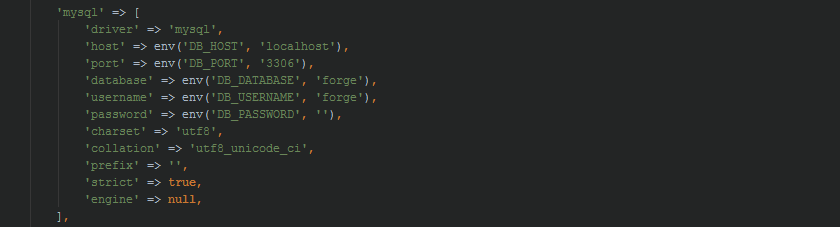
\includegraphics[height=2.3in]{Images/Implementation/MySQLConfig}
	\caption{Database Configuration for MySQL Databases} \label{fig:DatabaseConfig}
\end{figure}

\subsection{Migrations}
Migrations in Laravel are used to build database tables, and act as a database version control system, ``allowing a team to easily modify and share the application's database schema'' \cite{Laravel:Migrations}. The use of migrations not only allows for the database to be replicated anywhere the system is installed with ease but also simplifies the process of updating an existing table during the development process.  To create a migration, the \emph{make:migration}command provided by the Laravel Artisan utility is used. This command generates an empty template for a specified table. When creating a new table, the \emph{--create} argument is used whereas the \emph{--table} argument is used for modifying an existing table. The generated template contains an \emph{up} method, used for adding new columns and index, and a \emph{down} method which reverses the changes produced by the \emph{up} method. Migrations are typically paired with Laravel's schema builder to easily build your application's database schema \cite{Laravel:Migrations}. The schema builder can be used to define the schema for the table using calls to PHP functions. Once the schema has been populated, the \emph{migrate} command can be used to run the migration and update the database. In the case of an error the users can revert to a previous version of the database using the \emph{migrate:rollback} command. It is always encouraged that major changes, such as adding new columns and adding indexes, are introduced using new migrations rather than rolling back and updating existing migrations. All database tables were created using Laravel migrations and are available in the code.

\begin{figure}[H]
	\centering
	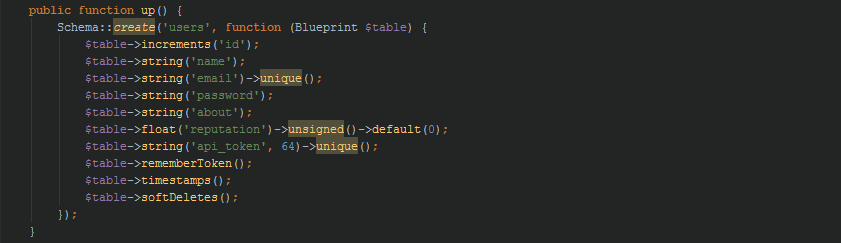
\includegraphics[height=2in]{Images/Implementation/UserMigration}
	\caption{Migration for creating Users table} \label{fig:UserMigration}
\end{figure}

Figure \ref{fig:UserMigration} shows the migration for the users table, which is used to store user information. The migration in the figure is not the final schema, and rather is the schema used during development. Additional migrations were used to add and modify columns in the table. As visible in the image, the schema builder can be used in the up method to define the structure of the table. Each migration schema contains an \emph{id} field, generated by calling the \emph{increments} method, and the \emph{created\_at} and \emph{updated\_at} timestamps, generated by calling the \emph{timestamps} method, by default. The \emph{increments} method is used for assigning an auto incrementing primary key, discussed later in the report, used for associating record through relationships. A \emph{deleted\_at} timestamp was added to all tables by calling the \emph{softDeletes} method. A range of other method such as \emph{string} and \emph{integer} can be used for creating more attributes. A full list of operations is available in the Laravel documentation \cite{Laravel:Migrations}. 

\subsection{Functional Dependencies and Constraints}
Majority of the foreign key constraints used in the database were setup with cascade delete and cascade update. This means that if a row in the referenced entity is removed or updated then any rows in the referencing entity which correspond to it are also updated or deleted \cite{TechOnTheNet:Cascading}. Some of the constraints followed the schema-bound dependencies by using the restrict keyword which prevents changes in the referenced entity if corresponding rows exist in the referencing entity. The use of all these techniques ensures that data is always kept consistent and no redundant data is introduced into the system.

\subsection{Security}
Security is of the upmost importance when it comes to a database which contains sensitive or personal information about individuals. For this reason, several measures should be taken into consideration to protect the database and the data in it from unauthorised access. The security threats and approaches taken to protect against them are discussed below.

\subsubsection{Access}
The first step to protecting the data is controlling who has access to the database and who is authorised to do what. This was achieved by creating separate SQL user accounts with different privileges. The database was then protected using a password to prevent any unauthorised access and only authorised users with a username and password would be able to access the database. Furthermore, each user was restricted so that the database would accept connections from the user if they were from a specified IP address. This meant that database connections could be restricted to just the web server and any users attempting to connect to the database from other machines would be denied access. When connecting to the database through PHP, root account was used for development purposes to prevent any restrictions but a separate account was used for production which was unable to modify the schema but could still query or modify the data.

\subsubsection{SQL Injection}
``SQL injection is a technique where malicious users can inject SQL commands into an SQL statement, via web page input'' \cite{W3Schools:SQL_Injection}. According to a report on 5,500 companies and 15,000 websites, almost half of these were vulnerable to serious security threats by XSS or SQL injection \cite{FirstPost:Vulnerabilities}. SQL injection can lead to all the data held in a database being made available. This is a serious threat as some of the data can be used to identify individuals and measures should be introduced to protect against this. One way to prevent SQL injection is by escaping all user input to prevent users from executing malicious queries. This is not a full fix for the issue as users can still enter data that can cause the system to malfunction. The alternative fix for this was using prepared queries which executes the query with placeholders and then binds the values later to retrieve the records. This method escapes SQL injection and prevents any unauthorised interaction with the database.

\subsection{Querying}
Laravel makes running queries extremely simple using either raw SQL statements, the fluent query builder, or the Eloquent Object-Relational Mapping (ORM) \cite{Laravel:Database}. For most part the Eloquent ORM approach was used to retrieve the result from the database but the approaches have been used in rare cases. All three approaches are outlined below.

\paragraph{Raw SQL}
With Laravel, raw SQL statements can be executed using the provided built-in classes. This removes the need to open a database connection, create SQL statements and bind parameters to these statements as this is all done automatically. For example, as shown in the example below, the user can run an SQL query to retrieve a user with a specific ID of 1 just by using the \emph{DB::select} method:

\begin{lstlisting}[language=php]
	$users = DB::select('SELECT * FROM users WHERE id = ?', [1]);
\end{lstlisting}

\noindent The above query will return an array of objects modelling the user entity in the database. Using this array, it is possible to loop through the array and access the properties of each user as \emph{\$user-$>$property}, where property may be any attribute such as username or email.

\paragraph{Query Builder}
The database query builder provides a convenient, fluent, and easy-to-use interface for creating and executing database queries \cite{Laravel:QueryBuilder}. The query builder can perform most operations supported by the database driver. One of the main advantages of using the query builder is that it uses PDO parameter bindings to prevent SQL injections, which means there is no need to sanitise user input. Using the query builder, one could retrieve the user with ID 1 by executing the following statement:

\begin{lstlisting}[language=php]
	$user = DB::table('users')->where('id', 1)->first();
\end{lstlisting}

\noindent The above query would fetch the result where the user ID matches the provided parameter and retrieve the first result. Once again, the result is returned as an object modelling the user entity and the properties can be accessed again as \emph{\$user-$>$property}.

\paragraph{Eloquent Object-Relational Mapping}
The Eloquent ORM included with Laravel provides an simple and elegant active record implementation for working with the database \cite{Laravel:Eloquent}. "Object-relational mapping (ORM) is a mechanism that makes it possible to address, access and manipulate objects without having to consider how those objects relate to their data sources" \cite{TechTarget:ORM}. Each database table has a corresponding "model" associated with it that is used database interactions and more specifically the table corresponding to a given model. Models allow the developer to query, insert, update, and delete records in the corresponding table as well as more complex operations such as joining tables. When querying the database using a model, Eloquent automatically instantiates and maps a model for each row in the result allowing the developer to utilise the models behaviour.

\begin{lstlisting}[language=bash]
	$ php artisan make:model Models/User
\end{lstlisting}

\noindent Creating a model is made simple again thanks to the Artisan utility. The command above will generate a User model in the \emph{app/Models} directory. Each Eloquent models extends the \emph{Illuminate/Database/Eloquent/Model} class which utilises the query builder for all interactions \cite{Laravel:Eloquent}. By default, Eloquent assumes that each table has a primary key field named \emph{id} and the \emph{created\_at} and \emph{updated\_at} timestamps but these can all be changed by toggling optional properties in the model. In order to use a model, the developer simply needs to import the model in the controller where it will be used. The user can simple execute the following command in order to retrieve the user with ID=1.

\begin{lstlisting}[language=php]
	$user = User::find(1);
\end{lstlisting}

\noindent The line of code above will return the \emph{User} model. It is again possible to access the model properties as \emph{\$user-$>$property}. The main change to be noticed here is that the user can actually update the properties and save the changes made by executing the following: \emph{\$user-$>$save()} \cite{Laravel:Eloquent}.  The image in figure \ref{fig:UserModel} shows the code for the \emph{User} model. As visible in the image, it is possible to add custom methods to the model which may be called when the model is returned as a result.

\begin{figure}[H]
	\centering
	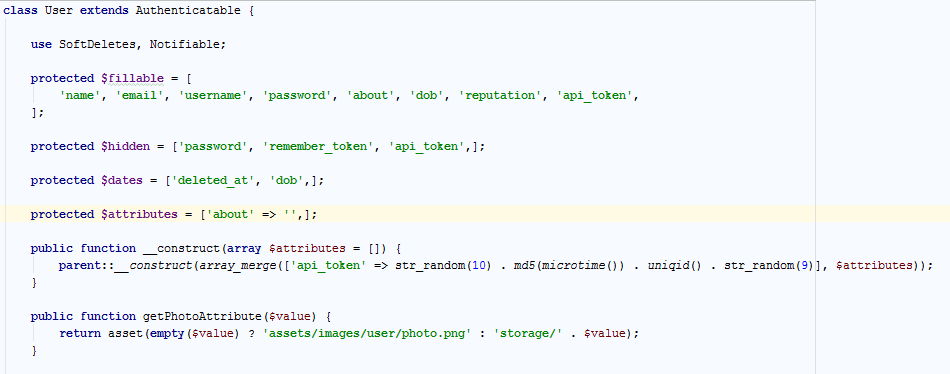
\includegraphics[width=1.0\textwidth]{Images/Implementation/UserModel}
	\caption{Users Eloquent ORM model} \label{fig:UserModel}
\end{figure}